To numerically solve a set of PDEs, iterative methods (finite difference, finite volume or finite element methods) are frequently used to approximate the solution through a discretized (step by step) phenomena. Thus, the continuous time and space domains are discretized so that a set of numerical computations are iteratively (time discretization) applied on a mesh (space discretization). In other words, the PDEs are transformed to a set of numerical computations applied at each time step on all elements of the discretized space domain. Among the numerical computations is found a set of numerical schemes, also called \textit{stencil computations}, and a set of local computations also needed to perform the simulation.
In the following Section, a formal definition of a \textit{stencil program} and its computations is given. Then, the different parallelization techniques which can be applied on such program, are presented.

%-------------------------------------
\subsection{Definitions}

A mesh $\mathcal{M}$ defines the discretization of the continuous space domain $\Omega$ of a set of PDEs and is defined as followed. 

\begin{mydef}
\textit{A mesh is a connected undirected graph $\mathcal{M}=(V,E)$, where $V$ is the set of vertices and $E$ the set of edges. The set of edges $E$ of a mesh $\mathcal{M}=(V,E)$ does not contain bridges.}
\end{mydef}

\begin{mydef}
$D_i$ is a set of elements of a mesh $\mathcal{M}=(V,E)$, constructed by a function $domain_i$ which defines a precise association between $V$ and $E$, $domain_i : V \times E \rightarrow D_i$.
\end{mydef}
For example, the set of cells $D_0$ in a Cartesian 2D mesh could be defined by exactly four vertices and four edges connected as a cycle. But we could also define another set of elements $D_1$ as the simple set of vertices $V$ etc.

A mesh can be structured (as Cartesian or curvilinear meshes), unstructured, regular or irregular (without the same topology for each element) and hybrid. 

\begin{figure}[!h]\begin{center}
  \resizebox{8cm}{!}{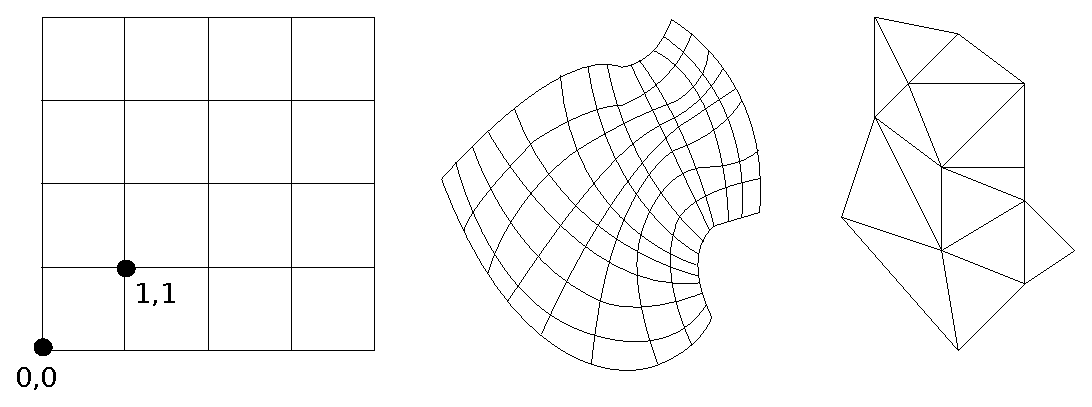
\includegraphics{./images/maillages.pdf}}
  \caption{From left to right, Cartesian, curvilinear and unstructured meshes.}
  \label{fig:mesh}
\end{center}\end{figure}

\begin{mydef}
The discretization of the continuous time domain $\mathcal{T}$ is denoted $T$ such that $\forall\mbox{ }t_i\mbox{, }t_{i+1} \in T\mbox{, }\exists\mbox{ }\Delta t \in \mathbb{R}$\mbox{, }$t_{i+1} = t_i + \Delta t$. Thus, $T$ is responsible for the iteration time steps of the numerical simulation. 
\end{mydef}

In a numerical simulation a set of data, or quantities, are applied onto the mesh and represent the set of values to compute, or to use, for computation.

\begin{mydef}
The set of data applied on the mesh is denoted by $\Delta$, such that $\delta \in \Delta$ is a function which associates each element $d \in D_i$ to a value $v \in V$, $\delta : D_i \rightarrow V$.
\end{mydef}
One can notice that in applied mathematics, the signature of $\delta$ would be $\delta : D_i \times T \rightarrow V$, however when programming a numerical simulation it is not wise to store all values of each time iteration.

\begin{mydef}
A numerical expression $\text{exp}$ is a function which represents how to compute, for an element $d \in D_i$, a data $w \in \Delta$ (written data) with a set $R \subset \Delta$ of input data (read data), $\text{exp} : R \times D_i \rightarrow w \times D_i$.
\end{mydef}

\begin{mydef}
A computation $c$ of a numerical simulation is defined as $c(R,w,D,\text{exp})$, where $R \subset \Delta, w \in \Delta$ and $\text{exp}$ a numerical expression. $D$ is one of the subsets $D_i \subset \mathcal{M}$, such that $w : D \rightarrow V$.
\end{mydef}
It has to be noticed that at each time iteration, all the elements of a mesh are computed. However, it happens that the computation of the mesh elements is splitted in different computations (for example the computation of the physical border). In this case additional $D_i$ can be specified for the mesh $\mathcal{M}$.

\begin{mydef}
The set of $n$ ordered computations of a numerical simulation is denoted $\Gamma = [c_i]_{0 \leq i \leq n-1}$, such that $\forall c_i,c_j$ with $i \leq j$, $c_i$ is computed before $c_j$, and $c_j$ can be computed only when $c_i$ is finished.
\end{mydef}

\begin{mydef}
Finally, a \textit{multi-stencil program} is defined by the quadruplet $\mathcal{MSP}(T,\mathcal{M},\Delta,\Gamma)$.
\end{mydef}
%If the number of computations in $\Gamma$ is $card(\Gamma)=n$, such that $\bigcup_{i=0}^{n-1}c_i = \Gamma$, then $\bigcup_{i=0}^{m-1}R_i \cup w_i \subseteq \Delta$.

As already mentioned, the ordered list $\Gamma$ can be composed of two different types of computations, stencil and local computations, which will be defined in the rest of this Section.

\begin{mydef}
The neighborhood $\mathcal{N}$ of an element $d \in D_i$ is a function to obtain a set of elements in any $D_k \subset \mathcal{M}$, $\mathcal{N} : D_i \rightarrow D_k \times D_k \times \dots$.
\end{mydef}
The function $\mathcal{N}$ is also sometimes called the \textit{stencil shape}, or the \textit{stencil} in applied mathematics. In this paper we distinguish a stencil shape from a \textit{stencil computation} defined as followed:

\begin{mydef}
A \textit{stencil computation} is defined as a quintuplet $s(R,w,D,\text{exp},\mathcal{N})$, where $R \subset \Delta, w \in \Delta$, $D$ is one the subsets $D_i$ and $w : D \rightarrow V$.
\end{mydef}
In a stencil computation $s$, $\forall d \in D$, the stencil numerical expression $\text{exp}$ is applied such that $w(d) = \text{exp}(R(d),R(\mathcal{N}(d))$. In this work, a stencil computation $s(R,w,D,\text{exp},\mathcal{N})$ always verifies $R \cap w = \emptyset$, otherwize an implicit numerical scheme has to be solve which is over the scope of this paper. As a result, the ordered list $\Gamma$ of a multi-stencil program can be composed of a set of stencil computations applied on one or more stencil shapes.

Figure~\ref{fig:ex} gives an example of a stencil computation $s(R,w,D,\text{exp},\mathcal{N})$, where $\mathcal{M}(V,E)$ is a two dimensional Cartesian mesh. A single domain $D$ is defined in this example and is composed of cells formed by a cycle of four vertices $v \in V$ and four edges $e \in E$. Furthermore, in this example $R=\{A\}$, $w=B$, and for $(x,y) \in D$ the neighborhood function is 
\begin{equation*}
\mathcal{N} : (x,y) \rightarrow \{(x,y+1),(x,y-1),(x+1,y),(x-1,y)\}.
\end{equation*}
Finally, the numerical expression of this example is 
\begin{equation*}
\text{exp}(A(x,y),A(\mathcal{N}(x,y)) = B(x,y) = A(x,y)+(A(x,y+1)+A(x,y-1)+A(x+1,y)+A(x-1,y))/4.
\end{equation*}

\begin{figure}[!h]\begin{center}
  \resizebox{8cm}{!}{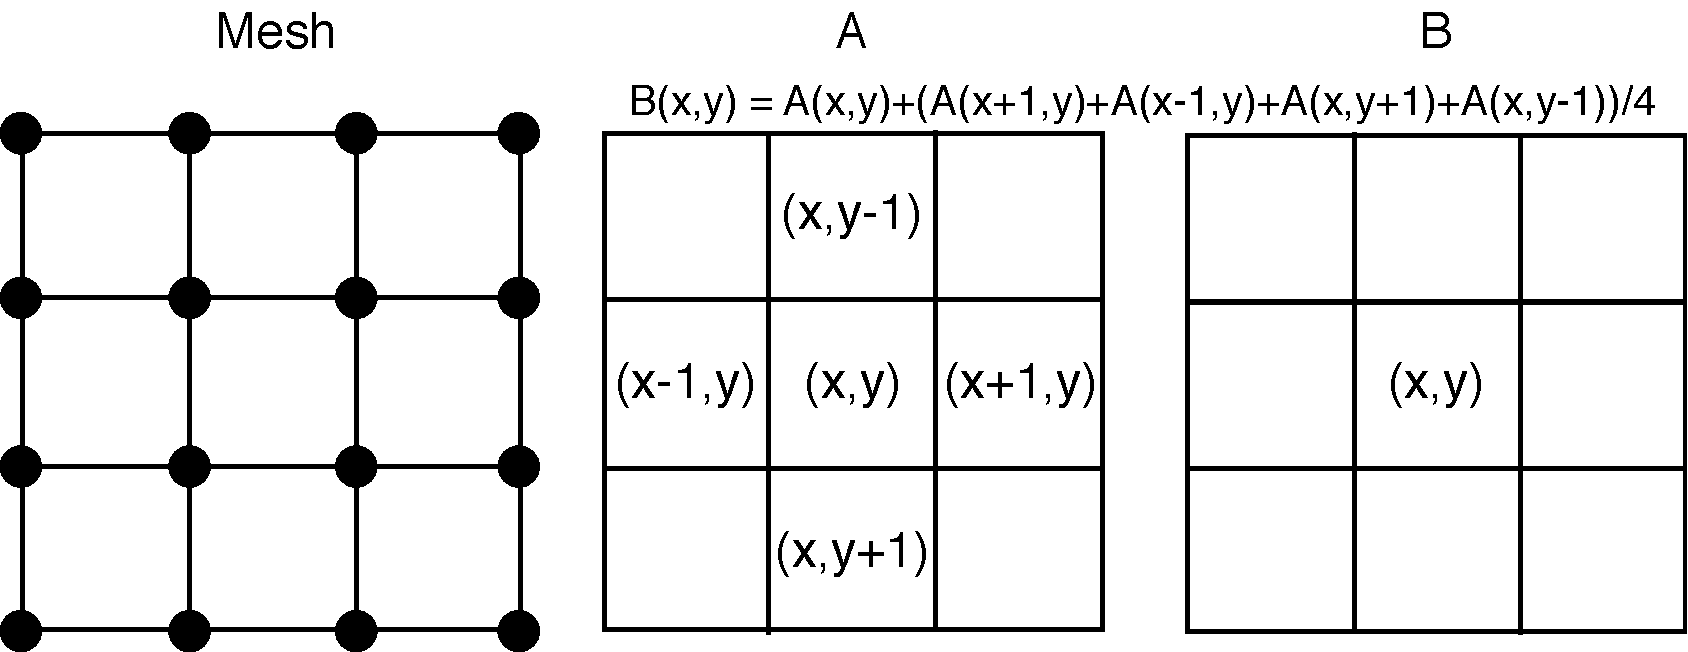
\includegraphics{./images/example.pdf}}
  \caption{Example of a stencil computation.}
  \label{fig:ex}
\end{center}\end{figure}

Finally, the second type of numerical computation is a local computation.
\begin{mydef}
A local computation is a quadruplet $l(R,w,D,\text{exp})$, where $e$ does not involve a neighborhood function $\mathcal{N}$.
\end{mydef}

A stencil program and stencil and local computations have been formally defined in this section. This formalism is used in the next Section to define two parallelization techniques of a multi-stencil program.

%-------------------------------------
\subsection{Parallelization}
\label{sect:parall}
Multi-stencil mesh-based numerical simulation can be parallelized in various ways and is an interesting kind of application to take advantage of modern heterogeneous HPC architectures, mixing clusters, multi-cores CPUs, vectorization units, GPGPU and many-core accelerators.

\paragraph{Coarse-grain data parallelism.} In a data parallelization technique, the idea is to split the data on which the program is computed in balanced sub-parts, one for each available resource. The same sequential program can afterwards be applied on each sub-part simultaneously, with some additioinal synchronizations between resources to update the data not computed locally, and thus to guarantee a correct result.

More formally, the data parallelization of a multi-stencil program $\mathcal{MSP}(T,\mathcal{M},\Delta,\Gamma)$ consists in, first, a partitioning of the mesh $\mathcal{M}$ in $p$ balanced sub-meshes (for $p$ resources) $\{\mathcal{M}_0,\dots,\mathcal{M}_{p-1}\}$. This step can be performed by an external graph partitionner~\cite{} and is not adressed by this paper. As a data is mapped onto the mesh, the set of data $\Delta$ is partitionned the same way than the mesh in $\{\Delta_0,\dots,\Delta_{p-1}\}$. The second step of the parallelization is to identify in $\Gamma$ the needed synchronizations between resources to update data, and thus to build a new ordered list of computations $\Gamma_{data}$.

\begin{mydef}
For $n$ the number of computations in $\Gamma$, and for $i,j$ such that $i<j<n$, a \textit{synchronisation} is needed between $c_i$ and $c_j$, denoted $c_i \pprec c_j$, if $c_j=s_j(R_j,w_j,D_j,\text{exp}_j)$, and $w_i \subset R_j$. Moreover, the data to update is $w_i \cap R_j = w_i$.
\end{mydef}

Actually, a synchronization can only be needed by the data read by a stencil computation (not local), and only if this data has been modified before, which means that it has been written before. This synchronization is needed because the neighborhood function $\mathcal{N}$ of a stencil computation involves values computed on different resources.

\begin{mydef}
A synchronization between two computations $c_i \pprec c_j$ is defined as a specific computation $\text{update}(w_i \cap R_j)=\text{update}(w_i)$.
\end{mydef}

\begin{mydef}
An \textit{updated-computation} a computation which needs a data synchronization before it can be performed. If $c_i \pprec c_j$, with $i<j$, the computation $c_j$ is transformed to an updated-computation $c^*_j(R_j,w_j,D_j,\text{exp}_j,\text{update}(w_i))$ such that $\text{update}(w_i)$ is performed before the evaluation of $exp_j$. The updated-computation can also be denoted as $c^*_j(c_j,\text{update}(w_i))$.
\end{mydef}

\begin{mydef}
The concatenation of two ordered lists of respectively $n$ and $m$ computations $l_1=[c_i]_{0 \leq i \leq n-1}$ and $l_2=[c'_i]_{0 \leq i \leq m-1}$ is denoted $l_1 \cdot l_2$ and is equal to a new ordered list $l_3=[c_0,\dots,c_{n-1},c'_0,\dots,c'_{m-1}]$.
\end{mydef}

\begin{mydef}
From the ordered list of computation $\Gamma$, a new ordered list $\Gamma_{data}$ is obtained from the call $\Gamma_{data} = T_{data}(\Gamma,0)$, where $T_{data}$ is the recursive function defined as
\begin{equation*}
T_{data}(\Gamma,i) = 
\begin{cases} 	[\Gamma[i]] \cdot T_{data}(\Gamma,i+1) & \mbox{if }\forall j\leq i\mbox{, } c_j \not\pprec c_i\\
				[c^*_i(\Gamma[i],\text{update}(\{w_k\})] \cdot T_{data}(\Gamma,i+1) & \forall k < i\mbox{, }c_k \pprec c_i\\
				[] & \mbox{if }i=|\Gamma|.
\end{cases}
\end{equation*}
\end{mydef}

The construction of $\Gamma_{data}$ implies that if a synchronization is needed it is always proceeded before the computation wich needs it. However, an optimization is possible to combine synchronizations together, and thus to synchronize more than one data at a time. If the number of synchronizations is reduced, final performance of the program will be better. For this reason, we define a reduction to apply to $\Gamma_{data}$, and which is performed as a post-transformation.

\begin{myprop}
Denoting four computations $c_l$, $c_k$, $c_i$ and $c_j$ of $\Gamma$, with $l<k$, $i<j$, and where $c_l \pprec c_k$ and $c_i \pprec c_j$. Then, computations $c_k$ and $c_j$ are tansformed to $c^*_k(c_k,update(w_l)$ and $c^*_j(c_j,update(w_i)$. If $i<k$, a single update call can be performed at $k$ such that $c^*_k(c_k,update(w_l\cup w_i)$, and in this case, the computation $c_j$ is not transformed.
\end{myprop}

\begin{proof}
By definition, the synchronization of $w_i$ can be performed between $c_i$ and $c_j$. As $i<k$ the computation $c_i$ is not performed between $k$ and $j$. As a result, the synchronization of $w_i$ can be performed between $c_i$ and $c_k$.
\end{proof}

In other words, for each synchronization in $\Gamma_{data}$, if the computation $c_i$ from which $c_j$ is synchronized occurs before the last synchronization, the two synchronizations can be reduced to one with the union of the data to update.

% We denote an function to insert at a precise position of a given ordered list, a computation $c_{up}$, as
% \begin{equation}
% \text{insert} : [c_k]_{0 \leq k \leq n-1} \times \text{position} \times c_{up} \rightarrow [c_0,\dots,c_{\text{position}-1},c_{up},\dots,c_{n-1}]
% \end{equation}

% The new ordered list of computations $\Gamma'$ is obtained from the insertion of the synchronizations at the good position. Algorithm~\ref{alg:gammaprime} illustrates how $\Gamma'$ is build.
% \begin{center}
% \begin{algorithm}
% $\Gamma' = \Gamma$\\
% $\text{offset} = 0$\\
% \For{$c_j \in \Gamma$}{
% 	\uIf{$c_j$ is a stencil}{
% 	\uIf{$\Gamma[c_0:c_j]==[]$}{
% 	$\text{insert}(\Gamma',0,\text{update}(R_j)$\\
% 	$\text{offset}++$\\
% 	}
% 	\uElse{
% 	\For{$c_i \in \Gamma[c_0:c_j]$}{
% 	\uIf{$c_i \pprec c_j$}{
% 	$\text{insert}(\Gamma',j+\text{offset},\text{update}(w_i \cap R_j)$\\
% 	$\text{offset}++$
% 	}
% 	}
% 	}
% 	}
% 	}
% \caption{Creation of $\Gamma'$ from $\Gamma$}
% \label{alg:gammaprime}
% \end{algorithm}
% \end{center}

 The final step of this parallelization is to run $\Gamma_{data}$ on each resource. Thus, for each resource $0 \leq k \leq p-1$ a multi-stencil program defined by
\begin{equation}
\mathcal{MSP}_k(T,\mathcal{M}_k,\Delta_k,\Gamma_{data}),
\end{equation}
is performed.

We denote this parallelization technique a coarse-grain data parallelization in contrast with the same technique applied to the finer level of a single computation. In this case, for a computation $c(R,w,D,\text{exp})$, the local domain $D$ is partitionned for $p$ resources $\{D_0,\dots,D_{p-1}\}$, and each resource $k$ is responsible for a sub-computation $c_k(R,w,D_k,\text{exp}')$.
%This finer data parallelization is particularly adapted to shared memory architectures (multi-cores, many-cores or GPUs), and in such case it does not require the addition of synchronizations because the computed element is local to the sub-domain $D_k$. Actually, if the computation is a stencil, the computation only read neighborhood elements but does not write them which does not require a synchronization, and if the computation is local nothing is read or written in the sub-domain of another resource. 
This finer data parallelization technique is not directly adressed by the work presented in this paper, but is exhibited, as it will be explained later. 

\paragraph{Task parallelism.}
A task parallelization technique is a technique to transform a program as a dependency graph of different tasks. A dependency graph exhibits parallel tasks, or on the contrary sequential execution of tasks. In a multi-stencil program a task is defined as a computation $c(R,w,D,\text{exp})$. As a result, the dependency graph of a multi-stencil program represents the dependencies between local and stencil computations of $\Gamma$.

\begin{mydef}
For two computations $c_i(R_i,w_i,D_i,e_i)$ and $c_j(R_j,w_j,D_j,e_j)$, with $i < j$, it is said that $c_j$ is data dependant from $c_i$, denoted $c_i\prec c_j$, if $w_i \cap R_j \neq \emptyset$. In this case, $c_i$ has to be computed before $c_j$. The binary relation $c_i\prec c_j$ represents a \textit{dependency}.
\end{mydef}

\begin{myprop}
The binary relation $\prec$ is not transitive. 
\end{myprop}

\begin{proof}
Considering three computations $c_0(R_0,w_0,D_0,e_0)$, $c_1(R_1,w_1,D_1,e_1)$ and $c_2(R_2,w_2,D_2,e_2)$, where $w_0\cap R_1 \neq \emptyset$ and $w_1\cap R_2 \neq \emptyset$. In this case two dependencies can be extracted $c_0 \prec c_1$ and $c_1 \prec c_2$. However, the dependency $c_0 \prec c_2$ is not true as $w_0\cap R_2 = \emptyset$.
\end{proof}

It has been proved that the binary relation $\prec$ is not transitive. This property is due to the fact that $\prec$ is defined as a data dependency between computations. A dependency chain, however, creates another type of dependency only due to time.

\begin{mydef}
For two computations $c_i(R_i,w_i,D_i,e_i)$ and $c_j(R_j,w_j,D_j,e_j)$, a time dependency is denoted $c_i \blacktriangleleft c_j$ and means that $c_i$ has to be computed before $c_j$.
\end{mydef}

As a result, the relation $\blacktriangleleft$ is more general than $\prec$.

\begin{myprop}
For two computations $c_i(R_i,w_i,D_i,e_i)$ and $c_j(R_j,w_j,D_j,e_j)$ such that $c_i \prec c_j$, $c_i \blacktriangleleft c_j$ is verified.
\end{myprop}

\begin{proof}
By definition $c_i \prec c_j$ means that $w_i\cap R_j \neq \emptyset$ and that $c_i$ has to computed before $c_j$. %Thus, the relation $c_i \prec c_j$ is stronger than $c_i \blacktriangleleft c_j$.
\end{proof}

\begin{myprop}
The binary relation $\blacktriangleleft$ is transitive. 
\end{myprop}

\begin{proof}
Considering three computations $c_0(R_0,w_0,D_0,e_0)$, $c_1(R_1,w_1,D_1,e_1)$ and $c_2(R_2,w_2,D_2,e_2)$, where $c_0 \blacktriangleleft c_1$ and $c_1 \blacktriangleleft c_2$. $c_0$ is computed before $c_1$ and $c_1$ is computed before $c_2$, as a result $c_0$ is computed before $c_2$ and the relation $c_0 \blacktriangleleft c_2$ is verified. 
\end{proof}

\begin{mydef}
A directed acyclic graph (DAG) $G(V,A)$ is a graph where the edges are directed from a source to a destination vertex, and where following the direction of edges, no cycle can be found from a vertex $u$ to itself. A directed edge is called an arc, and for two vertices $v,u \in V$ an arc from $u$ to $v$ is denoted $(\overset{\frown}{u,v}) \in A$.
\end{mydef}

From an ordered list of computations, a directed dependency graph $\Gamma_{task}(V,A)$ can be built finding all pairs of computations $c_i(R_i,w_i,D_i,e_i)$ and $c_j(R_j,w_j,D_j,e_j)$, with $i<j$, such that $c_i \blacktriangleleft c_j$. Those time dependencies can be found from pairs of data dependencies $c_i \prec c_j$.

\begin{mydef}
For two directed graphs $G(V,A)$ and $G'(V',A')$, the union $(V,A)\cup (V',A')$ is defined as the union of each set $(V\cup V', A \cup A')$.
\end{mydef}

\begin{mydef}
From an ordered list $\Gamma$ of computations $c(R,w,D,\text{exp})$, a directed dependency graph $\Gamma_{task}(V,A)$ is obtained from the call $T_{task}(\Gamma,0)$, where $T_{task}$ is the recursive function
\begin{equation*}
T_{task}(\Gamma,i) = 
\begin{cases} 	(\{\},\{\}) & \mbox{if }i=|\Gamma|\\
				(c_i, \{(\overset{\frown}{c_k,c_i})\mbox{, }\forall k < i \mbox{, } c_k\prec c_i \})\cup T_{task}(\Gamma,i+1) & \mbox{if }i<|\Gamma|
\end{cases}
\end{equation*}
\end{mydef}

This constructive function is possible because the input is an ordered list. Actually, if $c_k\prec c_i$ then $k<i$. As a result, $c_k$ is already in $V$ when the arc $(\overset{\frown}{c_k,c_i})$ is built. 

\begin{myprop}
The directed graph $\Gamma_{task}$ is an acyclic graph.
\end{myprop}

\begin{proof}
$\Gamma_{task}$ is built from $\Gamma$ which is an ordered and sequential list of computations. Moreover, each computation of the list $\Gamma$ is associated to a vertex of $V$, even if the same computation is represented more than once in $\Gamma$. As a result it is not possible to go back to a previous computation and to create a cycle.
\end{proof}

Using the function $T_{task}$ to build $\Gamma_{task}$, however, duplication of dependencies may occur because of the transitivity of the relation $\blacktriangleleft$. Actually, as the relation $\prec$ verifies the relation $\blacktriangleleft$, and as $\blacktriangleleft$ is transitive, if for three computations $c_k(R_k,w_k,D_k,e_k)$, $c_i(R_i,w_i,D_i,e_i)$ and $c_j(R_j,w_j,D_j,e_j)$, with $k<i<j$ and where $c_k \prec c_i$, $c_i \prec c_j$ and $c_k \prec c_j$, then the transitivity $c_k \blacktriangleleft c_j$ is verified because of the relations $c_k \blacktriangleleft c_i$ and $c_i \blacktriangleleft c_j$. However, $c_k \blacktriangleleft c_j$ is also directly represented by the binary relation $c_k \prec c_j$. As a result, a duplication of the dependency is created in $\Gamma_{task}$. In Figure~\ref{fig:duplication} an example of duplication is given for the relation $c_1 \blacktriangleleft c_4$.

\begin{figure}[h!]
\begin{center}
\begin{tikzpicture}[shorten >=1pt, node distance=2cm, on grid, auto]
   \node[component] (c0) at (0,0) {$c_0$};
   \node[component] (c1) at (1,0) {$c_1$};
   \node[component] (c2) at (2,0) {$c_2$};
   \node[component] (c3) at (3,0) {$c_3$};
   \node[component] (c4) at (4,0) {$c_4$};
 
  \path[->]
    (c0) edge node {} (c1)
    (c1.east) edge node {} (c2)
    	 edge [bend right=50] node [swap] {} (c4)
    (c2) edge node {} (c3)
    (c3) edge node {} (c4);
  \end{tikzpicture}
  \caption{Useless duplication of the dependency $c_1 \blacktriangleleft c_4$}
  \label{fig:duplication}
\end{center}
\end{figure}

Another view of the relations $\prec$ and $\blacktriangleleft$ is that $c_i\blacktriangleleft c_j$ in $\Gamma_{task}$ is a path from $c_i$ to $c_j$ of any size, while $c_i \prec c_j$ is a path of size $1$ from $c_i$ to $c_j$. And in any case a path in the graph represents a time dependency between computations. Scheduling a graph dependency which do not contains duplication of information is easier. For this reason, we define a reduction to apply to $\Gamma_{task}$, and which is performed as a post-transformation. In the example of Figure~\ref{fig:duplication} the dependency represented by the path $c_1 \blacktriangleleft c_2 \blacktriangleleft c_3 \blacktriangleleft c_4$ gives more information than the one directly represented by $c_1 \prec c_4$. The proposed reduction is based on this property.

\begin{mydef}
The dependency graph $\Gamma_{task}(V,A)$ is reduced to the dependency graph $\Gamma_{task}(V,A')$, where $A' \subseteq A$. A direct arc $(\overset{\frown}{c_i,c_j})$, $i<j$, of $A$, which means that $c_i \prec c_j$, is included in $A'$ if no longer path $c_i \blacktriangleleft c_j$ exists in $A$ because of transitivity.
\end{mydef}

%For each resource and from the previous parallelization technique has been obtained a multi-stencil program $\mathcal{MSP}_k(T,\mathcal{M}_k,\Delta_k,\Gamma')$. A new stencil program $\mathcal{MSP}_k(T,\mathcal{M}_k,\Delta_k,\Gamma'')$ is built to combine the previous coarse-grain data parallelization technique to a task parallelization technique.

%The set of tasks to perform in a $\mathcal{MSP}_k$ is the set of computations $\Gamma'$. From $\Gamma'$ the task graph $\Gamma''$ is built and is a directed acyclic graph (DAG). We denote the DAG $\Gamma''(V,A)$, where $V$ is the set of vertices of the DAG, and $A$ is the set of directed edges between vertices. Each vertex of the set $V$ of $\Gamma''$ corresponds to a computation in the ordered list $\Gamma'$, and the set $A$ is built from the definition of a dependency.

%In Algorithm~\ref{alg:gammasecond}, $\text{adj}$ denotes the adjacency list of the DAG $\Gamma''$, which associates two vertices together to form a directed edge. %In other words, Algorithm~\ref{alg:gammasecond} illustrates the creation of the set of directed edges $A$, thus th creation of $\Gamma''$.

% \begin{center}
% \begin{algorithm}
% $adj = \emptyset$\\
% \For{$c_j \in \Gamma'$}{
% 	\For{$c_i \in \Gamma'[c_0:c_j]$}{
% 	\uIf{$c_i<c_j$}{
% 	adj.append($(c_i,c_j)$)
% 	}
% 	}
% 	}
% \caption{Creation of $\Gamma''$ from $\Gamma'$}
% \label{alg:gammasecond}
% \end{algorithm}
% \end{center}

%However, the adjacency list obtained from Algorithm~\ref{alg:gammasecond} contains dummy edges...

\paragraph{Hybrid parallelism.}
It is also possible to combine coarse-grain data and task parallelization techniques to get hybrid parallelism, sometimes more efficient on hybrid architectures. A coarse-grain data parallelism creates for $k$ resources $k$ multi-stencil computations $\mathcal{MSP}_k(T,\mathcal{M}_k,\Delta_k,\Gamma_{data})$, where $\Gamma_{data}$ is built from an ordered list of computations and is itself an ordered list of computations $c$ and updated-computations $c^*$. On the other hand, the task parallelization technique builds, from an ordered list of computation, a graph dependency $\Gamma_{task}$. As a result $T_{data}$ and $T_{task}$ can be composed to build $\Gamma_{hybrid}$ such as $k$ multi-stencil programs
\begin{equation*}
\mathcal{MSP}_k(T,\mathcal{M}_k,\Delta_k,\Gamma_{hybrid})
\end{equation*}
are responsible for an hybrid parallelization of a multi-stencil program. The set of computation $\Gamma_{hybrid}$ is a dependency graph between computations $c$ and updated-computations $c^*$ and can be built from the call to 
\begin{equation*}
T_{task}(T_{data}(\Gamma,0),0).
\end{equation*}
